\chapter{Usage of the Software OpenDiHu}\label{sec:usage}

\Opendihu{} is an Open Source software framework for static and dynamic multi-physics problems that can be solved with the Finite Element Method. 
It was developed essentially by the author as part of this work with some code contributions given by Aaron Krämer, Nehzat Emamy and Felix Huber from the \emph{Institute for Parallel and Distributed Systems} and the \emph{Institute of Applied Analysis and Numerical Simulation}.
We use it to simulate the multi-scale models presented in the last chapter: biophysical problems describing biomechanics and neurophysiology of the musculoskeletal system.

In this chapter, we introduce basic concepts and present details on the usage of our software. The next chapter \cref{sec:implementation} continues with a discussion of internal software aspects and gives details on how the different algorithms and solvers are implemented.

We begin this chapter with an explanation of the design goals in \cref{sec:design_goals}. Next, \cref{sec:usage} showcases how to setup simulation programs for various scenarios based on examples. Some biochemical models are conveniently formulated and shared in the bioengineering community using the CellML description language \cite{Cellml2003}. \Cref{sec:usage_cellml} gives more details on the usage of CellML models in our software. Finally, \cref{sec:output_file_formats} discusses various output formats and compatible tools for visualization.

\section{Design Goals}\label{sec:design_goals}

Simulations of complex multi-scale models require the combination of tailored numerical solution schemes. Spatial mesh resolutions and timestep widths should be chosen carefully to avoid instabilities and to allow the completion of useful simulation time spans in feasible runtimes.
Numerical solvers on 1D, 2D and 3D meshes have to be coupled and the data should be mapped between these meshes. 

The simulations should be parallelized to efficiently exploit today's hardware and reduce the runtime to a minimum. Parallel runs should be performant on small workstations, on larger compute servers and on supercomputers. 

Scenarios for different use cases should be possible, ranging from convenient debugging with simple physics and small problem sizes to large runs with highly resolved meshes and comprehensive models. Schemes for input and output of the data should be available for all of these use cases. Established community standards for models, such as the CellML description, and output file formats should be considered.
The configuration of models and solver parameters should be flexible, well organized and properly documented to allow an efficient workflow.

%Input and output have to be processed in proper data formats for different purposes, ranging
% efficient storage and visualization of large datasets

In addition to this feature list from a user perspective, further requirements can be formulated from a developer perspective.
The program code should be modular, structured and well documented to allow discovery, reuse and extension in the future. The implemented solvers should compute correct results, which should be testable to preserve correctness during code changes.

OpenDiHu aims to fulfill these requirements.
%With these user and developer requirements in mind we develop our software framework named \opendihu{}.
%In the different contexts of reporting and software development, the presented capitalized name and an all lower case version of the name are used, respectively. 
The name originates from the Digital Human project that aimed to advance the field of biomechanics by \say{providing new possibilities to improve the understanding of the neuromuscular system by switching from small-sized cluster model problems to realistic simulations on HPC clusters} \cite{DihuWeb}. The software framework contributes to this goal.
%The software has been introduced in a publication \cite{Maier2019}.

In the following, we concretize the requirements and formulate design goals to guide the software development.
The design goals can be summarized under the keywords \emph{usability}, \emph{performance} and \emph{extensibility}. They span the field of requirements from user centric properties to developer centric properties.

\subsection{Usability}
Usability is defined in ISO 9241-11 \cite{ISO9241} as \say{the extent to which a product can be used by specified users to achieve specified goals with effectiveness, efficiency, and satisfaction in a specified context of use.}  
We target at users with a basic understanding of biophysics, numerics, programming and command line usage in Linux. 
The specified goals include---in increasing complexity---to reproduce results of existing studies,  analyze the simulation results,  adjust parameters of existing simulations to achieve different model behavior, conduct studies over a set of different parameters,  exchange numerical schemes to improve stability or efficiency, combine implemented parts of models to a new multi-physics model, and implement new solvers for completely new physics. The context of use lies in scientific and educational studies. 
%The program can be run in serial or in parallel on a small-scale compute server or compute cluster or on a supercomputer.

We base the usage of the framework on command line programs and scripts and do not include a graphical user interface (GUI). A GUI would need to present an abstract, simplified layer of the simulation setup, that reduces the understanding of the actual process. Furthermore, it would be difficult to keep a GUI up to date with all functionality that gets implemented in the software over time. The advantage of a command-line-only-program is, that it can be easily used in automated studies with different parameter combinations. Furthermore, it simplifies usage on remote computers such as compute clusters and supercomputers.

In this context, good usability is ensured by using the Python programming language for the configuration of the simulation.
The computational code of every simulation is written in C++ and compiled to a hardware specific executable, which enables good computational performance. The user can configure all parameters using Python scripting. The Python3 interpreter is linked into the C++ program such that the configuration script can be parsed at runtime when the simulation program is executed.

Thus, users can organize the simulation settings using their own variable names.
Users can compute derived parameter values within the settings script, they have the flexibility to organize the settings in multiple files, and define own command line parameters for every example. Input data and results of the simulation can be preprocessed and postprocessed directly in the Python settings script.

\subsection{Perfomance}
The second design goal is to achieve good performance.
OpenDiHu satisfies this goal by supporting parallel execution on the one hand and by providing efficient algorithms on the other hand. 

Simulations can be run on distributed and shared memory systems. The computational domains are mainly discretized with structured meshes, that can easily be partitioned into subdomains for multiple processes. For large scale simulations on multiple cores, the input data such as node positions can be specified in a distributed way. Hence, every process only needs to know its own portion of the whole simulation and the total amount of data can exceed the storage capabilities of a single compute core.

Efficient algorithms involve efficient numerical solvers such as multigrid or conjugate gradient schemes and optimized data handling within the software framework.
We use the external library \emph{PETSc} \cite{petsc-efficient1997} for the parallel storage of vectors and matrices and for linear algebra operations. PETSc provides a large collection of preconditioners, linear and nonlinear solvers that can be chosen at runtime. At the same time, it offers low-level access to the locally stored data, which, e.g., allows us to optimize data transfer between different arrays.

For multiscale models, good performance can only be achieved, when the data transfer between different solvers is also efficient. Using profiling tools, runtime hotspots in various simulation programs were regularly identified and evaluated. The portions of code, that use  most runtime should be the actual computations and not memory allocations or data transfer operations.
Using these insights, the framework was constructed in an efficient way, e.g., by avoiding repeated memory initializations and expensive copy operations whenever possible.

\subsection{Extensibility}
By extensibility, we refer to the possibility to add solvers for new physical processes to the existing framework.
This is facilitated when existing components of the framework are documented and can be reused. 

On the highest level, existing simulation programs using models in the CellML format can be altered to solve different physics by exchanging the CellML model. For example, model extensions of the active mechanical behavior of the half-sarcomeres can be implemented in the corresponding CellML model and without changing the C++ code.

It is also possible to use the adapters in OpenDiHu for the numeric coupling library \emph{preCICE} \cite{precice} to numerically couple  software packages to OpenDiHu. The surface coupling adapter allows to couple external mechanics solvers and exchange displacements and traction forces. The volume coupling adapter allows, e.g., to use the electrophysiology solver in OpenDiHu and couple it with external models of the muscle or other organs.

On the next level, which still does not require changing the C++ core, the modular building blocks of model solvers such as timestepping schemes for the solution of ODEs, operator splittings or coupling schemes can be newly combined for different behavior.

Solving other models, for which no solver has been designed, involves adding new code to the software framework.
The solvers in OpenDiHu use structures like function spaces consisting of meshes and basis functions, linear system solvers and output writers for data output, which are self-contained and get reused at different locations in the framework. A completely new model, e.g., an electro-magnetic description of electrophysiology would require a dedicated new solver class. 
Two template classes exist in OpenDiHu that can be copied and adjusted to create such a new solver for either transient or static problems.

Polymorphism concepts of the C++ programming language such as object orientation (OO) and template meta-programming (TMP) allow to write generic algorithmic code that gets specialized for the particular use-cases at runtime (OO) or at compile time (TMP). For example, most of the solvers are independent of the type of mesh they operate on. Similarly, an explicit timestepping scheme has the same definition regardless whether it solves a 0D subcellular model with a high-dimensional state vector or a 3D linear elasticity formulation discretized by Finite Elements, where the solution is a vector field with three components.
These concepts help to reuse existing structures in OpenDiHu.

%\subsection{Overview of this Chapter}
%Usage of the software and its implementation reflects the properties presented in the previous sections. More %details are given in the remainder of this chapter. TODO

%Details are given on the implementation, the underlying algorithms, and the application from a user's perspective. For selected topics, a comparison to other existing simulation frameworks for biomechanical problems such as OpenCMISS is given.
%The aim of this chapter is to describe how the software is used and how it is implemented. We begin with an introduction of its usage in \cref{sec:usage}. The remainder of this chapter addresses the implementation. \Cref{sec:data_handling_with_petsc} presents details on the data handling based on the library PETSc. \Cref{sec:fem_matrices_and_bc} describes the assembly of Finite Element matrices and shows an algorithm for Dirichlet boundary conditions.  TODO

\section{Usage of OpenDiHu}\label{sec:usage}
We begin with a aspects of OpenDiHu that are relevant from a user's perspective. This section outlines the basic organization of the repository in \cref{sec:organization_of_the_directory}, the installation procedure in \cref{sec:installation} and demonstrates the usage of given example scenarios in \cref{sec:exemplary_usage_1,sec:exemplary_usage_2,sec:exemplary_usage_3}. \Cref{sec:summary_of_existing_solver_classes} summarizes all available solver classes.

\subsection{Organization of the Repository}\label{sec:organization_of_the_directory}
The complete OpenDiHu is contained in a single git repository which is hosted on github at \url{https://github.com/maierbn/opendihu}. In addition, the documentation is hosted on the \say{Read the Docs} website under \url{https://opendihu.readthedocs.io} \cite{opendihuWeb}. This documentation is split into a user and a developer documentation. The user part includes introductory information such as installation instructions, a description of most of the existing simulation scenarios with images of the results, instructions how to build and run them and a complete reference of the settings of all available solvers.

\begin{figure}
\centering
%\begin{lstlisting}[columns=fullflexible,breaklines=true,postbreak=\mbox{\textcolor{gray}{$\hookrightarrow$}\space}]

\begin{framed}
\begin{subfigure}[t]{0.45\textwidth}%
\begin{Verbatim}[fontsize=\small]
opendihu
├── core
│   └── src
├── examples
│   ├── debug
│   ├── laplace
│   ├── poisson
│   ├── diffusion
│   ├── solid_mechanics
│   ├── fiber_tracing
│   └── electrophysiology
│       ├── cellml
│       ├── monodomain
│       ├── fibers
│       ├── multidomain
│       ├── neuromuscular
│       ├── meshes
│       └── input

\end{Verbatim}
\end{subfigure}
\begin{subfigure}[t]{0.45\textwidth}%
\begin{Verbatim}[fontsize=\small]

├── dependencies
│   ├── petsc
│   ├── python
│   ├── scons
│   ├── scons-config
│     ...
├── doc
│   ├── sphinx
│   ├── sympy
│     ...
├── scripts
│     ...
├── testing
│   └── unit_testing
├── SConstructGeneral
├── user-variables.scons.py
├── Makefile
└── config.log
\end{Verbatim}
\end{subfigure}
\end{framed}
\caption{Contents of the main opendihu directory.}%
\label{fig:directory_structure}%
\end{figure}

After cloning the git repository, the directory has the contents shown in \cref{fig:directory_structure}, which will be explained in the following.
The software consists of a core library, that provides all functionality such as solvers and data handling. In addition, examples are created, that set up specific simulation scenarios and import the required solvers by linking to the core library. 

The subdirectory \code{core/src} contains all C++ code that is compiled into the core library. This source code consists of approximately \num{90000} code lines, \num{24000} blank lines and \num{19000} comment lines contained in approximately 700 files and structured in a directory tree with approximately 70 total subdirectories.

The \code{examples} directory contains all simulation scenarios that are packaged with Open-\break DiHu. Each of the approximately 65 examples demonstrates how to solve a different model, often in several variations with different parameters and numerical schemes. 
%Each example is a collection of one or several small C++ source code files that define the solvers and the corresponding Python settings files. 
The examples are grouped by the subdirectories shown in \cref{fig:directory_structure} in different categories: technical examples for debugging, scenarios for solving the Laplace, Poisson and diffusion equations, various solid mechanics models, fiber tracing examples that can be used to generate meshes as described in \cref{sec:generation_of_meshes_for_multiscale}, and the electrophysiology models. 
The electrophysiology examples are further structured as given in \cref{fig:directory_structure} with increasing complexity: 
subcellular CellML model solvers (0D) in the subdirectory \code{cellml}, 
solvers for the monodomain equation (1D), i.e., electrophysiology on a single fiber in \code{monodomain}, 
models with multiple 1D fibers also coupled with the 3D EMG model or muscle contraction model in \code{fibers}, 
the same but with the multidomain model in \code{multidomain}, 
and models of motor neurons coupled with fibers and multidomain models in the \code{neuromuscular} directory. 

The directory \code{meshes} contains scripts and raw data to generate all meshes needed by the simulations. The directory \code{input} collects all input files that are used in any example, e.g., cellml models, meshes, and text files that specify MU assignments and firing times. Because this directory contains large files, it is not included in the git repository but hosted on a separate file server.

The \code{dependencies} directory contains the source files and installations of all external packages, such as PETSc in \code{petsc}, the Python3 interpreter in \code{python}, and the SCons related packages in \code{scons} and \code{scons-config}. This directory will be automatically filled with more subdirectories during the installation procedure.

The \code{doc} directory collects various documents and mathematical derivations that help to understand certain solvers. For example, the directory \code{doc/sphinx} contains the whole online documentation, which is hosted on the \say{Read The Docs} website \cite{opendihuWeb} and built using the reStructuredText markup language and the Sphinx generation system. The \code{doc/sympy} directory contains python scripts with the derivation of various equations using the symbolic math package SymPy.

Various utility Python scripts are stored in the directory \code{scripts}. Users should add this directory to the \code{$\$$PATH} environment variable in their system such that the scripts can be invoked from the command prompt. For example, the \code{catpy} and \code{plot} scripts list and visualize python-based output files of simulations, other scripts can be used to inspect and manipulate binary mesh files.

The directory \code{testing/unit_testing} contains the code for all unit tests. Furthermore, the files that exist directly under the top level \code{opendihu} directory are relevant for the build system, which will be explained in the next section.

\subsection{Installation}\label{sec:installation}
% scons

The installation procedure involves three steps: First, the dependencies, i.e., all required external packages have to be located. Second, the OpenDiHu core library is compiled and linked. Third and optionally, unit tests are compiled, linked and executed.

The first step consists of finding the location of each dependency, determining the corresponding header and library files that are needed for inclusion and linking, and potentially determining special compiler or linker flags. The step can be configured to fit the individual system setup and use case by taking into account already existing dependencies and enabling or disabling optional packages.

The second step compiles the source code and links it to all dependencies that were collected in the first step. The result is a static library, which contains the functionality of OpenDiHu in executable form. To run a particular simulation, an additional program with a small source code file has to be written, compiled and linked to this library.

For the compilation of unit tests in the third step, a similar action is performed. The step builds and links three unit testing executables that are subsequently run with one, two and six processes and conduct various functional tests of the implementation.

Currently, the following fifteen dependencies are used with OpenDiHu: the standard for shared-memory parallelisation \emph{MPI} \cite{openmpi}, the data handling and numerics library \emph{PETSc} \cite{petsc-efficient1997,petsc-user-ref,petsc-web-page}, the \emph{Python interpreter} \cite{python3}, a set of \emph{Python packages} including \emph{NumPy} \cite{numpy}, \emph{SciPy} \cite{scipy} and \emph{Matplotlib} \cite{matplotlib} among others, a \emph{Base64} compression library \cite{base64}, the unit testing framework \emph{Googletest} \cite{googletest}, the compile-time differentiation toolbox \emph{SEMT} \cite{gutterman2004symbolic,semt}, the parallel file I/O library \emph{ADIOS2} \cite{adios2}, the vectorization toolbox \emph{Vc} \cite{vc2012,Kretz2015} and its newer version \emph{std-simd} \cite{hoberock2016working}, the library for parallel time integration with multigrid \emph{XBraid} \cite{xbraid-package}, the solver and converter for CellML models \emph{OpenCOR} \cite{OpenCOR2015}, the XML parser \emph{libxml2} \cite{libxml2}, the coupling library \emph{preCICE} \cite{precice} and the logging library \emph{Easylogging++} \cite{easyloggingpp}. The build system has to install these dependencies and possibly cope with different sets of available versions and prerequisites.

% This action usually relies on configuration files or command line options to manually enable or disable certain dependecies and to manually specify their locations.

Popular build systems exist that facilitate the three mentioned installation step, e.g., CMake, GNU Autoconf and SCons. CMake uses a three-step process of configuration, generation and building, which requires users to have the corresponding know-how. Autoconf creates a configure script that relies on command line options instead of a configuration file for all settings. 

Considering the usability goal for OpenDiHu, we chose the build system SCons as it requires little previous knowledge and can read its settings from a python based configuration file. SCons performs the three steps of the installation procedure by a single command. Packages that are not yet installed are downloaded and installed automatically, using transparent bash commands.
Furthermore, the SCons build system itself is packaged along with our software and, thus, no additional installation steps are required to begin the build process (apart from checking that some essential packages such as a compiler and an MPI implementation are available).

SCons allows to both specify the installation configuration and extend the functionality by using the Python scripting language. Based on the scons-config package \cite{sconsconfig}, we added functionality to detect and automatically download the dependencies that are required for OpenDiHu. For some dependencies, multiple versions are tried if the first attempt fails, e.g., for Python and PETSc.
This adds robustness for different systems and typically allows to setup OpenDiHu on a new Linux computer by only executing a single \say{\code{scons}} command.

The top-level files listed in \cref{fig:directory_structure} are related to the build system. The file \code{SConstruct}\code{General} contains python code that defines various flags for the usual build targets: the \code{release} targets creates optimized and hardware-specific binaries, the \code{debug} target disables optimization and adds debugging symbols to the executables, other debugging targets produce intermediate outputs after the  preprocessing, assembly or optimization stages. All options are documented in the help text of the build system.

The \code{user-variables.scons.py} file contains the configuration and can be adjusted by the user to enable or disable certain packages or features. The \code{Makefile} contains convenient shortcuts for longer build command, e.g., the command \say{\code{make}} builds the debug and release targets and runs the unit tests. During installation, all text output and progress information is appended to the log file \code{config.log}. If the installation fails, this file contains all information that is required to track down the respective issue.

After the installation and build step of the core library, individual simulation scenarios can be developed and executed. The place for the code of these simulations is in the \code{examples} subdirectory, where numerous predefined simulation scenarios are given. In the following, we demonstrate how to use OpenDiHu and, more specifically, we present the structure and configuration of a simulation program by considering three of these examples in increasing complexity: a Laplace problem in \cref{sec:exemplary_usage_1}, a simulation of muscle contraction in \cref{sec:exemplary_usage_2} and a simulation of the neuromuscular system in \cref{sec:exemplary_usage_3}.

\subsection{Exemplary Usage: Laplace Problem}\label{sec:exemplary_usage_1}
% Laplace example
Every simulation consists of a single C++ source file that gets compiled to an executable program and a Python file that defines all settings for the simulation. The example considered in the following solves a 2D Laplace problem and is located in the directory \code{examples/laplace/laplace2d}. The considered C++ source file is \code{src/laplace_structured.cpp} and the corresponding Python settings file is \code{settings_lagrange_quadratic.py}. The contents of the two files are listed in \cref{fig:laplace_example_source,fig:laplace_example_settings}. The directory additionally contains code for other scenarios that have different parameters and discretizations.

After compilation by the \say{\code{scons}} command, an executable is created in the \code{build_release} subdirectory of the example. In this directory, the simulation can be run with the following command:
\begin{lstlisting}[columns=fullflexible,breaklines=true,postbreak=\mbox{\textcolor{gray}{$\hookrightarrow$}\space}]
  ./laplace_structured ../settings_lagrange_quadratic.py
\end{lstlisting}
Here, the first item is the program name. We pass the filename of the settings file as the first command line argument. 
%For some examples, additional arguments can be given, those are accessible from within the Python settings script and can be used to adjust parameters.

\Cref{fig:laplace_example_source} lists the full C++ source code of this example. \Cref{code:c0l1} includes the main header file of opendihu, which makes all functionality available. The rest of the source file contains the definition of the \code{main} function. \Cref{code:c0l9} defines the context object \code{settings}, which uses the command line arguments given by \code{argc} and \code{argv}. This line invokes the Python interpreter on the Python settings file and stores all parameters in the \code{settings} object.

\Cref{code:c0l12,code:c0l13,code:c0l14,code:c0l15,code:c0l16,code:c0l17} define an object named \code{equationDiscretized}, which is of the \code{Finite}\code{ElementMethod} class located in the \code{SpatialDiscretization} namespace. The new object uses the settings object that was defined before.

The \code{FiniteElementMethod} class takes several class template arguments enclosed in angle brackets. The first in \cref{code:c0l13} specifies the mesh type, which, in this 2D example, is a structured deformable mesh of dimension two. Furthermore, \cref{code:c0l14} specifies quadratic Lagrange basis functions and \cref{code:c0l15} specifies Gauss quadrature with three Gauss points per dimension. The argument in \cref{code:c0l16} defines the equation that is discretized by this finite element method class, which, in this case, is the static Laplace equation $Δ\bfu = 0$.

In \cref{code:c0l20}, the solver is executed, performs the computation and writes the configured output files. The program finally returns in \cref{code:c0l22}.

% laplace2D c++ source
\begin{figure}
\centering
\begin{framed}
%\begin{Verbatim}[fontsize=\small]
\begin{lstlisting}[basicstyle=\small\ttfamily,commentstyle=\color{gray},numbers=left]
  #include <cstdlib>
  #include "opendihu.h" $\label{code:c0l1}$

  int main(int argc, char *argv[])
  {
    // 2D Laplace equation 0 = du^2/dx^2 + du^2/dy^2
    
    // initialize and parse settings from input file
    DihuContext settings(argc, argv);   $\label{code:c0l9}$
    
    // define the tree of solvers (here only one FEM solver)
    SpatialDiscretization::FiniteElementMethod<   $\label{code:c0l12}$
      Mesh::StructuredDeformableOfDimension<2>,   $\label{code:c0l13}$
      BasisFunction::LagrangeOfOrder<2>,          $\label{code:c0l14}$
      Quadrature::Gauss<3>,                       $\label{code:c0l15}$
      Equation::Static::Laplace                   $\label{code:c0l16}$
    > equationDiscretized(settings);              $\label{code:c0l17}$
    
    // run the simulation
    equationDiscretized.run();  $\label{code:c0l20}$
    
    return EXIT_SUCCESS;    $\label{code:c0l22}$
  }
\end{lstlisting}
%\end{Verbatim}
\end{framed}
\caption{Example source file of an OpenDiHu solver for the 2D Laplace problem.}%
\label{fig:laplace_example_source}%
\end{figure}

The problem to be solved is parametrized by the settings file \code{settings_lagrange_}\code{quadratic.py}, which is listed in \cref{fig:laplace_example_settings}. The code in this file can use all features of the Python scripting language. For example, in \cref{code:c1l5}, the \emph{NumPy} numerics packages is imported and its sine function is used in \cref{code:c1l11,code:c1l14}. The print statement in \cref{code:c1l16} is executed in the for loop in \cref{code:c1l7} and produces informational output about boundary condition values during execution. 

The settings file has to define the variable \code{config} to be a Python dictionary, i.e., an associative container data structure. This dictionary contains the parameter names and values that are required by the solver in the C++ program. 
In \cref{fig:laplace_example_settings}, the \code{config} dictionary is defined in \cref{code:c1l18,code:c1l19,code:c1l20,code:c1l21,code:c1l22,code:c1l23,code:c1l24,code:c1l25,code:c1l26,code:c1l27,code:c1l28,code:c1l29,code:c1l30,code:c1l31,code:c1l32,code:c1l33,code:c1l34,code:c1l35,code:c1l36,code:c1l37,code:c1l38,code:c1l39,code:c1l40,code:c1l41,code:c1l42,code:c1l43,code:c1l44,code:c1l45,code:c1l46,code:c1l47,code:c1l48,code:c1l49,code:c1l50,code:c1l51,code:c1l52}. It contains global options such as filenames of log files in \cref{code:c1l19,code:c1l20,code:c1l21,code:c1l22} followed by specific options for the Finite Element method object in \cref{code:c1l24,code:c1l25,code:c1l26,code:c1l27,code:c1l28,code:c1l29,code:c1l30,code:c1l31,code:c1l32,code:c1l33,code:c1l34,code:c1l35,code:c1l36,code:c1l37,code:c1l38,code:c1l39,code:c1l40,code:c1l41,code:c1l42,code:c1l43,code:c1l44,code:c1l45,code:c1l46,code:c1l47,code:c1l48,code:c1l49,code:c1l50}. The exact meaning of all parameters is documented in the online documentation \cite{opendihuWeb} and also sketched by the comments in the file. Some parameters will be presented in the following.

The parameter set consists of mesh parameters in \cref{code:c1l25,code:c1l26,code:c1l27,code:c1l28}, problem parameters in \cref{code:c1l31,code:c1l32,code:c1l33,code:c1l34}, 
solver parameters in \cref{code:c1l37,code:c1l38,code:c1l39,code:c1l40,code:c1l41,code:c1l42,code:c1l43,code:c1l44} and output writers in \cref{code:c1l47,code:c1l48,code:c1l49,code:c1l50}. 
The mesh in this scenario is a cartesian grid on the unit square. The number of elements is specified by the parameter \code{`nElements`}. The number of elements in $x$ and $y$-directions is given by the variables \code{nx} and \code{ny}, which are defined in \cref{code:c1l1} of the settings file. 

The parameter \code{`inputMeshIsGlobal`} is relevant for parallel execution. Its value specifies, whether all parameters apply to the global problem (\code{True}) or to a local subdomain (\code{False}). If the given example is executed by four processes, the mesh will have $10\times 10$ elements, as specified by \code{nx} and \code{ny}. 
However, if \code{`inputMeshIsGlobal`} is set to \code{False}, each of the $2\times 2$ subdomains would create a mesh of this size, yielding a total mesh of $20 \times 20$ elements. Instead of the cartesian grid, it is also possible to define the node positions of every element. Then, it is beneficial to only specify the data for the own subdomain on each process for meshes with large numbers of elements and large numbers of processes.

This example problem uses Dirichlet boundary conditions. Values of a sine curve are prescribed at the boundaries $y=0$ and $y=1$ of the unit square. \Cref{code:c1l31} of the settings file sets the boundary conditions to the variable \code{bc}. This variable is defined in the loop before the \code{config} dictionary in \cref{code:c1l6,code:c1l7,code:c1l8,code:c1l9,code:c1l10,code:c1l11,code:c1l12,code:c1l13,code:c1l14,code:c1l15,code:c1l16}. The \code{bc} variable itself is a dictionary that specifies the prescribed values for every degree of freedom. 

\Cref{code:c1l38,code:c1l39} specify the employed preconditioner and solver by strings that are given to the solver library PETSc. Thus, all linear solvers available in PETSc can be used.
Error tolerances on the residual norm and a maximum number of iterations can be specified. It is also possible to dump the system matrix, right hand side and solution vectors to a text file or a MATLAB readable file using the options in \cref{code:c1l42,code:c1l43}.

Output of the simulation results is configured by specifying a list of output writers in \cref{code:c1l47,code:c1l48,code:c1l49,code:c1l50}. The considered example has the two output writers with formats \code{`Paraview`} and \code{`PythonFile`}. The former writes files that can be visualized by the software \emph{ParaView}, the latter outputs files that can be easily parsed with a Python script. Both output writers either generate binary or human-readable files, depending on the \code{`binary`} option. Binary files have smaller file sizes and are used for large datasets. The human-readable text files make it is easier to debug the output.

After the program has been run, the \code{out} subdirectory contains the two output files created by the output writers. The Python based file can be visualized using the command \say{\code{plot}}, which is also provided by OpenDiHu. \Cref{fig:laplace_example_plot} shows the resulting \emph{Matplotlib} visualization. The figure shows that the Dirichlet boundary conditions for $y=0$ and $y=1$ are met and the solution is a harmonic function.

% laplace2D settings
\begin{figure}
\centering
\begin{framed}
\begin{lstlisting}[basicstyle=\footnotesize\ttfamily,language=Python,commentstyle=\color{gray},numbers=left]
  nx = 10;       ny = nx          # number of elements   $\label{code:c1l1}$
  mx = 2*nx + 1; my = 2*ny + 1    # number of nodes    $\label{code:c1l2}$
                                                        $\label{code:c1l3}$
  # specify boundary conditions                         $\label{code:c1l4}$
  import numpy as np       $\label{code:c1l5}$
  bc = {}                    $\label{code:c1l6}$
  for i in range(mx):        $\label{code:c1l7}$
    x = i/mx                 $\label{code:c1l8}$
                                $\label{code:c1l9}$
    # bottom line                   $\label{code:c1l10}$
    bc[i] = np.sin(x*np.pi)       $\label{code:c1l11}$
                                   $\label{code:c1l12}$
    # top line                        $\label{code:c1l13}$
    bc[(my-1)*mx + i] = np.sin(x*np.pi)       $\label{code:c1l14}$
                                              $\label{code:c1l15}$
    print("{}, bc: {}, {}".format(i, bc[i], bc[(my-1)*mx + i]))       $\label{code:c1l16}$
                                                                             $\label{code:c1l17}$
  config = {                                                                      $\label{code:c1l18}$
    "solverStructureDiagramFile":     "solver_structure.txt",      # diagram file $\label{code:c1l19}$
    "logFormat":                      "csv",     # "csv" or "json", format of log $\label{code:c1l20}$
    "scenarioName":                   "laplace", # scenario name for log file     $\label{code:c1l21}$
    "mappingsBetweenMeshesLogFile":   None,      # a log file about mappings      $\label{code:c1l22}$
    "FiniteElementMethod": {                                                      $\label{code:c1l23}$
      # mesh parameters                                                           $\label{code:c1l24}$
      "nElements":                   [nx, ny],   # number of elements in x and y  $\label{code:c1l25}$
      "inputMeshIsGlobal":           True,       # if nElements is a global number$\label{code:c1l26}$
      "physicalExtent":              [1.0, 1.0], # physical domain size           $\label{code:c1l27}$
      "physicalOffset":              [0, 0],     # physical location of origin    $\label{code:c1l28}$
                                                                                  $\label{code:c1l29}$
      # problem parameters                                                        $\label{code:c1l30}$
      "dirichletBoundaryConditions": bc,         # Dirichlet BC as dict           $\label{code:c1l31}$
      "dirichletOutputFilename":     None,       # output file for Dirichlet BC   $\label{code:c1l32}$
      "neumannBoundaryConditions":   [],         # Neumann BC                     $\label{code:c1l33}$
      "prefactor":                   1,          # constant prefactor c in $\textcolor{gray}{c\Delta u}$   $\label{code:c1l34}$
                                                                                  $\label{code:c1l35}$
      # linear solver parameters                                                         $\label{code:c1l36}$
      "solverType":                  "gmres",    # linear solver scheme           $\label{code:c1l37}$
      "preconditionerType":          "none",     # preconditioner scheme          $\label{code:c1l38}$
      "relativeTolerance":           1e-15,      # stopping criterion, rel. tol.  $\label{code:c1l39}$
      "absoluteTolerance":           1e-10,      # stopping criterion, abs. tol.  $\label{code:c1l40}$
      "maxIterations":               1e4,        # maximum number of iterations   $\label{code:c1l41}$
      "dumpFormat":                  "default",  # format for data dump           $\label{code:c1l42}$
      "dumpFilename":                None,       # filename for dump              $\label{code:c1l43}$
      "slotName":                    None,       # connector of solver            $\label{code:c1l44}$
                                                                                  $\label{code:c1l45}$
      # output writers                                                            $\label{code:c1l46}$
      "OutputWriter" : [                                                          $\label{code:c1l47}$
        {"format": "Paraview",   "filename": "out/laplace", "binary": False},     $\label{code:c1l48}$
        {"format": "PythonFile", "filename": "out/laplace", "binary": False},     $\label{code:c1l49}$
      ]                                                                           $\label{code:c1l50}$
    }                                                                             $\label{code:c1l51}$
  }                                                                               $\label{code:c1l52}$
\end{lstlisting}
\end{framed}
\caption{Python settings file of the Laplace example corresponding to the source file in \cref{fig:laplace_example_source}.}%
\label{fig:laplace_example_settings}%
\end{figure}

% plot of Laplace solution
\begin{figure}[H]
  \centering%
  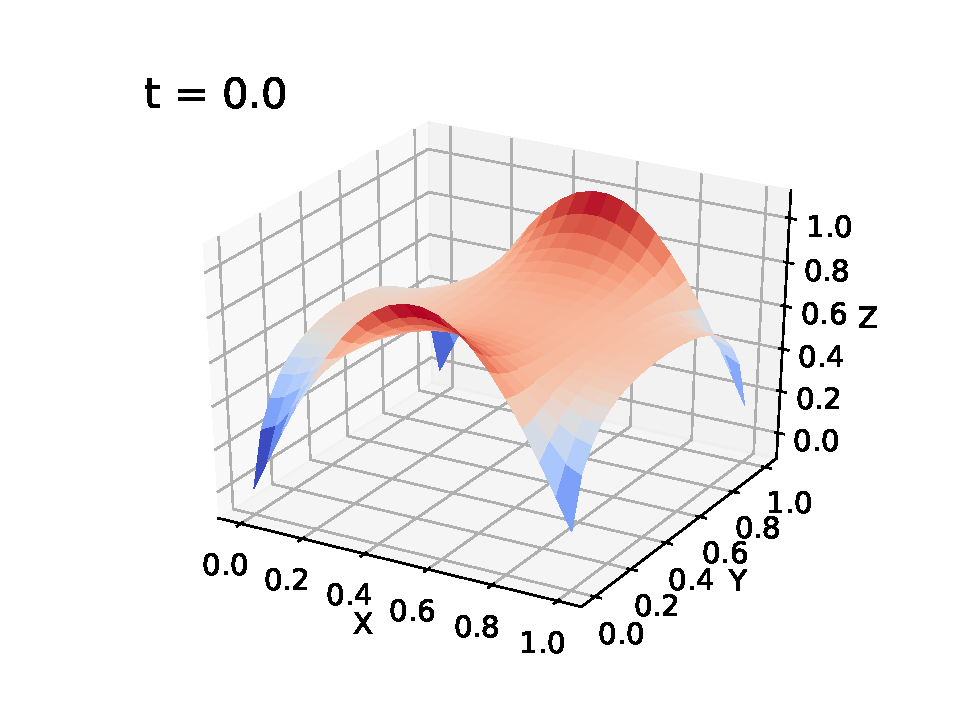
\includegraphics[width=0.7\textwidth]{images/implementation/laplace_plot.pdf}%
  \caption{Visualization of the solution of the exemplary 2D Laplace problem. The plot was created using the \code{plot} command on the output of the \code{PythonFile} output writer.}%
  \label{fig:laplace_example_plot}%
\end{figure}

\subsection{Exemplary Usage: Multidomain Model With Solid Mechanics}\label{sec:exemplary_usage_2}
% with multidomain, first show multidomain excerpt, then full solver_structure

The next example to be studied is a simulation of electrophysiology and muscle contraction. It uses the multidomain model on the muscle and body fat domains and bidirectionally couples the nonlinear solid mechanics model. The example is located in the directory \code{examples/electrophysiology/multidomain/multidomain_contraction}.

% multidomain_contraction C++ source
\begin{figure}
\centering
\begin{framed}
%\begin{Verbatim}[fontsize=\small]
\begin{lstlisting}[basicstyle=\scriptsize\ttfamily,commentstyle=\color{gray},numbers=left]
  #include <cstdlib>
  #include "opendihu.h"     $\label{code:c2l2}$

  int main(int argc, char *argv[])
  {
    // 3D multidomain coupled with contraction
    
    // initialize everything, handle arguments and parse settings from input file
    DihuContext settings(argc, argv);       $\label{code:c2l9}$
    
    typedef Mesh::StructuredDeformableOfDimension<3> MeshType;    $\label{code:c2l11}$

    Control::Coupling       $\label{code:c2l13}$
    <
      OperatorSplitting::Strang<          $\label{code:c2l15}$
        Control::MultipleInstances<     // subcellular model  $\label{code:c2l16}$      
          TimeSteppingScheme::Heun<       $\label{code:c2l17}$
            CellmlAdapter<                $\label{code:c2l18}$
              57,71,  // nStates,nAlgebraics: 57,71 = Shorten, 4,9 = Hodgkin Huxley     $\label{code:c2l19}$
              FunctionSpace::FunctionSpace<MeshType,BasisFunction::LagrangeOfOrder<1>>  $\label{code:c2l20}$
            >  
          >
        >,
        TimeSteppingScheme::MultidomainWithFatSolver<       // multidomain    $\label{code:c2l24}$
          SpatialDiscretization::FiniteElementMethod<       // FEM for initial potential flow    $\label{code:c2l25}$
            MeshType,                                       $\label{code:c2l26}$
            BasisFunction::LagrangeOfOrder<1>,
            Quadrature::Gauss<3>,
            Equation::Static::Laplace                            $\label{code:c2l29}$
          >,
          SpatialDiscretization::FiniteElementMethod<       // anisotropic conduction      $\label{code:c2l31}$
            MeshType,                                            $\label{code:c2l32}$
            BasisFunction::LagrangeOfOrder<1>,
            Quadrature::Gauss<5>,
            Equation::Dynamic::DirectionalDiffusion
          >,
          SpatialDiscretization::FiniteElementMethod<       // isotropic conduction in fat layer     $\label{code:c2l37}$
            MeshType,                                             $\label{code:c2l38}$
            BasisFunction::LagrangeOfOrder<1>,
            Quadrature::Gauss<5>,
            Equation::Dynamic::IsotropicDiffusion
          >
        >   $\label{code:c2l43}$
      >,
      MuscleContractionSolver<          // solid mechanics $\label{code:c2l45}$
        Mesh::CompositeOfDimension<3>     $\label{code:c2l46}$
      >
    > problem(settings);     $\label{code:c2l48}$
    
    problem.run();  $\label{code:c2l50}$
    
    return EXIT_SUCCESS;
  }
\end{lstlisting}
%\end{Verbatim}
\end{framed}
\caption{Source code of the simulation program that computes the multidomain model coupled with the solid mechanics model.}%
\label{fig:example_multidomain_source}%
\end{figure}

\Cref{fig:example_multidomain_source} shows the source code of the C++ file. The overall structure of the code is the same as in the previous Laplace example: \Cref{code:c2l2} includes the OpenDiHu header, the main function consists of the definition of a settings object in \cref{code:c2l9}, the definition of the solver in \crefrange{code:c2l13}{code:c2l48} and its execution in \cref{code:c2l50}. The only difference is the definition of the solver, which contains more nested class templates.

The problem is numerically solved by computing the multidomain model, transferring the activation parameter $\gamma$ from the multidomain mesh to the elasticity mesh, computing the solid mechanics model, and then mapping the deformed geometry back to the multidomain mesh. This compute cycle repeats in every timestep. This coupling between two models is performed by the \code{Control::Coupling} class defined as the outer-most solver in \cref{code:c2l13}. It nests the two solvers of the model parts: The first is the class named \code{OperatorSplitting::Strang} in \cref{code:c2l15}. It computes the multidomain electrophysiology model. The second class is the \code{MuscleContractionSolver} in \cref{code:c2l45}. It calls the solid mechanics solver and incorporates the activation and active stress term.

The multidomain model itself is computed using two coupled solvers. As formulated in \cref{sec:discretization}, a Strang operator splitting is used that alternates between solving the subcellular model and the electric conduction part of the multidomain model. In the code, these two parts are defined in \cref{code:c2l16} and \cref{code:c2l24}. As can be seen, the first part that solves the subcellular model consists of the three nested classes in \cref{code:c2l16,code:c2l17,code:c2l18}. The inner-most is the \code{CellmlAdapter}, which loads and executes a DAE model description from a CellML file. Its template arguments are the number of states and number of algebraic variables in \cref{code:c2l19} and the type of the function space in \cref{code:c2l20} used for spatial discretization.
The CellML model is solved by the enclosing Heun timestepping scheme in \cref{code:c2l17}. Because we need to solve the subcellular model for every compartment $k \in 1,\dots,N_\text{MU}$, a \code{MultipleInstances} class is used in \cref{code:c2l16}, which encloses the timestepping scheme and applies it on the domains for every compartment.

The second part of the multidomain model is the electric conduction in the intracellular, extracellular and body fat domains. It corresponds to solving the linear system of equations given in \cref{sec:discretization_body_domain}. This is done in OpenDiHu by the \code{MultidomainWithFatSolver} defined in \crefrange{code:c2l24}{code:c2l43}. It can be seen, that it nests three classes of type \code{FiniteElementMethod}. 

The first one in \cref{code:c2l25} is used to initially solve a potential flow problem, from which the fiber direction can be estimated. This approach \cite{Choi2013} is also used in the fiber generation algorithms described in \cref{sec:generation_of_fiber_meshes}. As a result, we get the anisotropy direction in the 3D domain, which is needed to define the anisotropic intracellular conduction tensors $\bfsigma_i^k$. As the problem to be solved is a Laplace problem, the equation to be discretized by the class is defined accordingly in \cref{code:c2l29}.

The second and third nested Finite Element classes are defined in \cref{code:c2l31,code:c2l37}. They define the isotropic electric conduction in the muscle domain and the anisotropic electric conduction in the fat domain and are used to set up the stiffness and mass matrices for these subproblems.

Several meshes are involved in the definition of this example. As described in \cref{sec:electric_conduction_body_domain}, the computational domain consists of a muscle domain and a fat domain. Both domains are discretized by a 3D structured mesh, which is given as \code{MeshType} in \cref{code:c2l11}. This type is referenced for the subcelullar model in \cref{code:c2l20} and for the conduction parts in \cref{code:c2l26,code:c2l32,code:c2l38}. 
%Only in the anisotropic conduction class, it refers to the fat domain, in the other uses it specifies the muscle domain.
For the muscle contraction solver in \cref{code:c2l46}, we use a different, \say{composite} type of mesh. This type is a combination of the two structured meshes for the body and for the fat domain, as the whole tissue should be considered in the computation of the deformation.

% multidomain_contraction solver_structure
\begin{figure}
\centering
\begin{framed}
\begin{lstlisting}[basicstyle=\scriptsize\ttfamily,language=Python,commentstyle=\color{gray},numbers=left]
  config = {
    "scenarioName": "multidomain_contraction",
    "Solvers": {
      "potentialFlowSolver": {...},   $\label{code:c3l4}$
    },
    "Coupling": {                $\label{code:c3l6}$
      "timeStepWidth": 1e-3,
      "Term1": {            # multidomain     $\label{code:c3l8}$
        "StrangSplitting": {                  $\label{code:c3l9}$
          
          "Term1": {        # subcellular model      $\label{code:c3l11}$
            "MultipleInstances": {                    $\label{code:c3l12}$
              "nInstances": variables.n_compartments,    $\label{code:c3l13}$
              "instances": [        # settings for each motor unit     $\label{code:c3l14}$
              {
                "ranks": list(range(n_ranks)),    $\label{code:c3l16}$
                "Heun": {
                  "CellML" : {
                  }
                }
              } for compartment_no in range(variables.n_compartments)] $\label{code:c3l21}$
            },   $\label{code:c3l122}$
          }, 
          "Term2": {        # conduction term of multidomain      $\label{code:c3l24}$
            "MultidomainSolver": {
              
              "PotentialFlow": {                                   $\label{code:c3l27}$
                "FiniteElementMethod": {  
                  "solverName": "potentialFlowSolver",            $\label{code:c3l29}$
                },
              },                                                    $\label{code:c3l31}$
              
              "OutputWriter": [ $\label{code:c3l33}$
              ]
            },
          }
        },
      },
      "Term2": {        # solid mechanics    $\label{code:c3l39}$
        "MuscleContractionSolver": {
          
          # the actual solid mechanics solver
          "DynamicHyperelasticitySolver": {
           }
        }
      }
    }
  }
\end{lstlisting}
\end{framed}
\caption{Excerpt of the settings file for the multidomain and solid mechanics solver.}%
\label{fig:example_multidomain_settings}%
\end{figure}

The Python settings script, that corresponds to the C++ source file, is given in \cref{fig:example_multidomain_settings}. Only the main structure of the \code{config} dictionary is outlined and the details are left out. It can be seen, that the definition in this file has a hierarchical structure. It is the same tree-like structure as in the C++ source.

The settings for the top-level coupling scheme start in \cref{code:c3l6}. First, some settings related to the timestepping scheme itself are specified of which one, the timestep width, is shown. Then, the settings of the two nested solvers are listed under \code{`Term1`} in \cref{code:c3l8} and \code{`Term2`} in \cref{code:c3l39}. Similarly, also the nested Strang splitting scheme in \cref{code:c3l9} defines its two nested solvers under \code{`Term1`} (\cref{code:c3l11}) and \code{`Term2`} (\cref{code:c3l24}).

\Crefrange{code:c3l12}{code:c3l122} define settings for the \code{MultipleInstances} class, which holds separate instances of the subcellular solver for all motor units.
The number of instances is specified by the \code{`nInstances`} parameter. A list containing the particular parameters for each instance is given under the keyword \code{`instances`} in \crefrange{code:c3l14}{code:c3l21}. This construct is a Python list comprehension, an inline definition of list entries defined by the for loop in \cref{code:c3l21}. The nested specifications of parameters of the Heun and the CellML methods, not shown in \cref{fig:example_multidomain_settings}, depend on the iteration index \code{compartment_no} of this loop. 
Each of these instance gets computed by a defined set of processes, specified under the parameter \\\code{`ranks`} in \cref{code:c3l16}. In this multidomain example, all processes take part in the computation of all multidomain compartments and, thus, all instances of the \code{MultipleInstances} class are computed by all processes. The expression in \cref{code:c3l16} expands to a list \code{[0,1,2,...]} indicating all available processes.

% solvers
Specifications of the parameters for a \code{FiniteElementMethod} class, similar to the Laplace example considered in \cref{sec:exemplary_usage_1}, also appear in the example of this section, once for each of the three occurences of this class. The excerpt of the settings file in \cref{fig:example_multidomain_settings} shows one of these specifications, the \code{PotentialFlow} finite element method, in \crefrange{code:c3l27}{code:c3l31}. 
This \code{FiniteElementMethod} class shares its mesh and its linear solver with other classes. The mesh and the linear solver both have specific parameters that were listed as blocks in the settings file of the Laplace problem in \cref{fig:laplace_example_settings}. To avoid duplication of this information and to share linear solvers and meshes, these parameters are not repeated for every class, by which they are required. Instead, parameters for linear solvers and meshes can be specified globally at the beginning of the settings file and referenced at the locations in inner classes, when they are used. In the example settings in \cref{fig:example_multidomain_settings}, this is indicated for the linear solver. Its parameters are defined under the global \code{`Solvers`} keyword  in the beginning and the name \code{`potentialFlowSolver`} in \cref{code:c3l4}. These settings are referenced in the finite element method in \cref{code:c3l29} using the \code{`solverName`} keyword. Internally, only one solver object with the related data structures of PETSc is created and reused whereever the solver is referenced by its solver name.

The meshes use an analog approach, in which all meshes can be defined under a global \code{`Meshes`} keyword (not shown in \cref{fig:example_multidomain_settings}) and referenced in the solver objects by their \code{`meshName`}. This is helpful especially for meshes with a large number of node positions that can be specified once and reused throughout all solvers.

% output writers
The output of the results is written to files by output writers that are defined as shown in the previous Laplace example in \cref{fig:laplace_example_settings}. Almost all solver classes allow to configure associated output writers. In \cref{fig:example_multidomain_settings}, such output writer settings are listed in \cref{code:c3l33} within the multidomain solver. Additional output writers can be defined in the Heun scheme of the subcellular model and in the \code{MuscleContractionSolver} for the solid mechanics models. Each output writer outputs files with the solution variables of the respective solver. Different time intervals can be set for the writers to allow for different output frequencies of large data such as all subcellular model states and of smaller data such as the solid mechanics outputs.

% command
The following exemplary command can be used to run the program for this example:
\begin{lstlisting}[columns=fullflexible,breaklines=true,postbreak=\mbox{\textcolor{gray}{$\hookrightarrow$}\space}]
  mpirun -n 2 ./multidomain_contraction ../settings_multidomain_contraction.py very_coarse.py --end_time=10
\end{lstlisting}
Similar to the Laplace example in \cref{sec:exemplary_usage_1}, the program \code{./multidomain_contraction} is called with the settings file \code{../settings_multidomain_contraction.py} as its first argument. In addition, a second script, \code{very_coarse.py}, is given as second argument. This script gets loaded from within the Python settings script and defines a number of high-level parameters in a separate \code{variables} namespace. These parameters are then used in the settings file. For example, \cref{code:c3l13} of \cref{fig:example_multidomain_settings} uses the variable \code{n_compartments}, which is defined in the so called \emph{variables} file \code{very_coarse.py}. The file name refers to the coarse discretization that is chosen in the particular scenario.

The rationale of this second script is to summarize important parameter values in a smaller and easier readable file. Whereas the full settings file corresponding to \cref{fig:example_multidomain_settings} contains approximately 500 lines and a complex nested structure, the variables script only contains about 200 lines, mainly value assignments to parameters and descriptive comments. 

Several of these variables files exist in the \code{variables} subdirectory of the example. They define different scenarios for the given simulation such as different mesh resolutions or CellML model files. By exchanging the filename in the second argument of the command line, these different scenarios can be easily executed.

The last argument in the command, \say{\code{--end_time=10}}, gets also parsed by the python script. It allows to set the end of the simulation time span to the specified value via the command line. Other options are available to alter various parameters in this scenario. These command line arguments take precedence over the parameter values that are specified in the Python scripts. This type of command line argument makes it possible to easily conduct parameter studies, e.g., from bash scripts, where the program can be called with different parameter values.
The architecture involving a main settings file with all parameters in the hierarchical solver structure, a set of small variables files with dedicated parameter choices and the possiblity to override all parameters from the command line is present in most of the advanced examples in OpenDiHu.

Another thing to note is that the given command begins with \say{\code{mpirun -n 2}}, which instructs MPI to launch the program using two processes. Here, any other number is possible and a corresponding domain decomposition is computed automatically. The parallelism is only bounded by the number of available elements in the meshes.

\subsection{Data Connections in the Example of a Multidomain Model with Solid Mechanics}\label{sec:exemplary_usage_2b}

The control flow of a simulation program with nested solvers such as the coupled electrophysiology and muscle contraction model studied in the previous section is defined by the tree of solvers in the C++ source file. This structure is reflected in the Python settings file.
The corresponding data flow, which connects the solvers, is another important property that has to be specified.
To help with this step, the program generates a diagram of its data connections whenever the program stops (either after completing or when interrupted by the shell).

\Cref{fig:example_multidomain_solver_structure} shows such a solver structure diagram for the current example. It is given as a text file and visualizes data connections using only unicode characters. This is advantageous for computers that only provide remote access, such as compute clusters. 
On the left side, the tree of nested solvers is given. On the right side, lines indicate the corresponding data connections.

% multidomain_contraction solver_structure
\begin{figure}
\centering
\begin{framed}
\begin{Verbatim}[fontsize=\scriptsize\ttfamily,numbers=left]
The following data slot connection were given by the setting "connectedSlots":
  stress ¤ ──> ¤ g_mu  
   g_tot ¤ ──> ¤ g_in  

The following data slots were connected because the names appeared in both terms:
  lambda ¤ <─> ¤ lambda

Solver structure: 
├── Coupling  
│     (...)
│ ├── StrangSplitting                          ::::::::::::::           
│ │  data slots:                               ::::::::::::::           
│ │  [a] solution.wal_environment/vS           ├÷÷÷÷÷÷÷÷÷÷÷÷÷─── vm ¤0  x
│ │  [a] razumova/stress                       :├÷÷÷÷÷÷÷÷÷÷÷÷stress ¤1  x
│ │  [a] (P)razumova/L_S                       ::├÷÷÷÷÷÷÷÷÷÷÷lambda ¤2<──────────┐
│ │  [a] Vm^(i)_0                              :::├÷÷÷÷÷÷÷÷÷÷vm_old ¤3  x        │
│ │  [a] Vm^(i+1)_0                            ::::├÷÷÷÷÷÷÷÷÷vm_new ¤4  x        │
│ │  [a] active_stress_0                       :::::├÷÷÷÷÷÷÷÷─ g_mu ¤5  x        │
│ │  [a] activeStressTotal                     ::::::├÷÷÷÷÷÷÷ g_tot ¤6─────────┐ │
│ │                                            ::::::::::::::                  │ │
│ │ ├── MultipleInstances  ("Term1")           ::::::::::::::                  │ │
│ │ │ ├── Heun                                 ::::::::::::::                  │ │
│ │ │ │  data slots:                           ::::::::::::::                  │ │
│ │ │ │  [a] solution.wal_environment/vS       ├÷÷÷÷÷÷÷÷÷÷÷÷÷─── vm ¤0<────┬─┐ │ │
│ │ │ │  [a] razumova/stress                    ├÷÷÷÷÷÷÷÷÷÷÷÷stress ¤1───┐ │ │ │ │
│ │ │ │  [a] (P)razumova/L_S                     ├÷÷÷÷÷÷÷÷÷÷÷lambda ¤2  x│ │ │ │ │
│ │ │ │                                           :::::::::::            │ │ │ │ │
│ │ │ │ └── CellmlAdapter                         :::::::::::            │ │ │ │ │
│ │ │ └                                           :::::::::::            │ │ │ │ │
│ │ └                                             :::::::::::            │ │ │ │ │
│ │                                               :::::::::::            │ │ │ │ │
│ │ ├── MultidomainSolver  ("Term2")              :::::::::::            │ │ │ │ │
│ │ │  data slots:                                :::::::::::            │ │ │ │ │
│ │ │  [a] Vm^(i)_0                               ├÷÷÷÷÷÷÷÷÷÷vm_old ¤0<──┼─┘ │ │ │
│ │ │  [a] Vm^(i+1)_0                              ├÷÷÷÷÷÷÷÷÷vm_new ¤1───┼───┘ │ m
│ │ │  [a] active_stress_0                          ├÷÷÷÷÷÷÷÷─ g_mu ¤2<──┘     │ │
│ │ │  [a] activeStressTotal                         ├÷÷÷÷÷÷÷ g_tot ¤3  x      │ │
│ │ │  (...)                                          :::::::                  m │
│ │ └                                                 :::::::                  │ │
│ └                                                   :::::::                  │ │
│                                                     :::::::                  │ │
│ ├── MuscleContractionSolver                         :::::::                  │ │ 
│ │   ("Term2")                                       :::::::                  │ │
│ │  data slots:                                      :::::::                  │ │
│ │  [b] λ                                            ├÷÷÷÷÷÷lambda ¤0<────────┼─┘
│ │  [b] λdot                                          ├÷÷÷÷÷─ ldot ¤1  x      │
│ │  [b] γ                                              ├÷÷÷÷─ g_in ¤2<────────┘
│ │  [b] T (material traction).x                         ├÷÷÷──── T ¤3  x
│ │  [b] u.x                                              ├÷÷────── ¤4  x
│ │  [b] u.y                                               ├÷────── ¤5  x
│ │  [b] u.z                                                ├────── ¤6  x
│ │                                                                     
│ │ └── DynamicHyperelasticitySolver    
│ │     (...)                                
│ └                                                                     
└                                                                       
                                                                        
Connection Types:
  +··+   Internal connection, no copy
  ════   Reuse variable, no copy
  ───>   Copy data in direction of arrow
  ─m──   Mapping between different meshes

Referenced Meshes:
  [a] "3Dmesh", 3D structured deformable, linear Lagrange basis
  [b] "3Dmesh_elasticity_quadratic+3DFatMesh_elasticity_quadratic", 3D quadratic Lagrange basis
  [c] "3DFatMesh", 3D structured deformable, linear Lagrange basis
\end{Verbatim}
\vspace{-5mm}
\end{framed}
\caption{Solver structure diagram that shows the data connections of the solvers.}%
\label{fig:example_multidomain_solver_structure}%
\end{figure}

Each solver has a fixed number of \emph{data connector slots}. A data connector slot is a scalar field variable or one component of a vector-valued field variable on a certain mesh. In coupling or operator splitting schemes, values can be transferred from a data connector slot of the first solver to a data connector slot of the second solver. This data transfer either reuses the internal data structure, if possible or it involves a copy operation. Either way, after the transfer, the second solver knows the corresponding values of the first solver and can use them in subsequent computations.

Each field variable has a given, fixed name defined by the solver. The corresponding data connector slot can have a custom name with a maximum length of six character, which is assigned from the Python settings.
The diagram shows the field variable names on the left under the \say{data slots} lists of the solvers. The corresponding data connector slots are marked by the \say{¤} symbol and a slot number on the right. The custom name of the slot is written before the \say{¤} symbol.

For example, the \code{MuscleContractionSolver} listed in line 42 has field variables for the fiber stretch \code{$\lambda$}, contraction velocity \code{$\lambda$dot}, muscle activation \code{$\gamma$}, traction in material description \code{T} and displacements in $x$, $y$ and $z$-direction, \code{u.x}, \code{u.y} and \code{u.z}. As can be seen in \cref{fig:example_multidomain_solver_structure}, the first four data  slots correspondingly have the names \code{lambda}, \code{ldot}, \code{g_in} and \code{T}. The fiber stretch \code{$\lambda$} is a quantity that is computed by the solver, and the activation parameter \code{$\gamma$} is a field variable that is an input to the solver and used for the computation of the active stress. However, data connector slots make no distinction between input and output slots, they simply expose the corresponding field variable to be connected to other slots.

The Heun solver in line 22 that solves the subcellular model has three slots: the slot \code{vm} of the transmembrane voltage, the slot named \code{stress} of the active stress parameter $\gamma$ and the slot \code{lambda}, which is the input of the relative half-sarcomere length of the subcellular model.

The multidomain solver in line 32 has four slots: the slot \code{vm_old} exposes the field variable for $V_m^{(i)}$, the transmembrane voltage at the previous timestep. After solving the linear system of equations, the field variable $V_m^{(i+1)}$, which is connected to the slot \code{vm_new}, holds the transmembrane voltage for the next timestep. Another slot used for data input is \code{g_mu}, which retrieves the muscle activation parameter $\gamma$ from each compartment. The multidomain solver computes the resulting activation parameter at slot \code{g_tot} by the weighted sum over the $\gamma$ values at the intracellular compartments. 

In case of the multidomain solver, separate field variables exist for every compartment at the same data connector slot. The solver structure diagram in \cref{fig:example_multidomain_solver_structure} shows the field variables for slots 0 to 2 ending in \say{\code{_0}} for the compartment $k=0$. Similar field variables exist for $k=1,\dots,N_\text{MU}$, however, those are not shown in the diagram. Similarly, the Heun scheme in line 22 is nested in the \code{MultipleInstances} scheme in line 21. Here, the field variables that connect to the slots \code{vm}, \code{stress} and \code{lambda} also have different instances for every compartment. To resolve the ambiguity of multiple field variables of the same kind being associated with a single slot, every exposed field variable for data transfer has to be identified by its slot and potentially an array index within this slot.

In case of nested solvers, the parent solver class always exposes data connector slots of its children. For example, the \code{StrangSplitting} class in line 11 has no own slots, but exposes the slots of its two children. The slots with indices 0 to 2 are the same as the slots of its \code{`Term1`} in line 21, the slots 3 to 6 are identical to the \code{`Term2`}, the \code{MultidomainSolver} in line 32. These connections are indicated in the diagram by the dotted vertical connection lines.
Note that the outer-most solver always contains the slots of all nested solvers. In the example in \cref{fig:example_multidomain_solver_structure}, this is the outer \code{Coupling} scheme. The slot listing has been omitted in the visualization.

The actual connections between the data slots of different solvers are indicated by the arrows on the right hand side of the slots. Unconnected slots are marked by an \say{x}.
The data transfer behavior is as follows. Each coupling and operator splitting scheme has two nested solvers. The coupling scheme executes the first solver, transfers the data over the connected data slots from the first to the second solver, executes the second solver, and then transfers the data according to the connected slots from the second to the first solver. For the Strang splitting scheme, this data transfer happens twice per timestep, as defined by the splitting algorithm (cf. \cref{fig:strang_splitting}).

The interaction between the subcellular model and the multidomain model is given by the arrows between the Heun scheme in line 22 and the \code{MultidomainSolver} in line 32. After the solution of the subcellular model, the transmembrane voltage is transferred from slot 0 (\code{vm}) of the Heun scheme to slot 0 (\code{vm_old}) of the multidomain solver. At the same time, the stress is transferred from slot 1 (\code{stress}) to slot 2 (\code{g_mu}). After the linear system has been solved, the values for the new timestep are transferred back from slot 1 (\code{vm_new}) to slot 0 (\code{vm}).

At the outer \code{Coupling} scheme, after the electrophysiology model consisting of the subcellular and multidomain model parts have been solved, the active total stress is transferred from slot 6 (\code{g_tot}) in line 19 to the slot 2 (\code{g_in}) of the \code{MuscleContractionSolver}. Note that the starting slot \code{g_tot} is shared between \code{StrangSplitting} and \code{Multidomain}\code{Solver}, shown by the dotted vertical lines. Then, the solid mechanics model uses the activation value, computes new displacements and updates the slots \code{lambda} and \code{ldot}. The value in \code{lambda} is transferred back to slot 2 of the \code{StrangSplitting}, where it is shared with the subcellular model. The value of the slot \code{ldot}, which is the contraction velocity, is not used here, however, some subcellular CellML models make use of this value. In such a case, the corresponding connection line can be added.

In addition to the \code{lambda} slot, the \code{MuscleContractionSolver} updates the muscle geometry with the new deformed configuration. This occurs outside of data connector slots using defined relationships or mappings between the elasticity and electrophysiology meshes.
Reasons for this exception are, first, that a mesh is not owned by a solver class in the same way as other data, e.g., as a solution vector. And second, the geometry information is different from normal field variables. Changing the geometry of a mesh, e.g, invalidates finite element system matrices.

% meshes
Each field variable is associated with a mesh, which is referenced by \code{[a]} and \code{[b]} in front of the field variable names. The referenced meshes are listed at the bottom of the diagram in line 64. The reference \code{[a]} corresponds to the mesh in the muscle domain used for the subcellular and multidomain models. The reference \code{[b]} is the composite mesh of both muscle and fat domain used for the solid mechanics problem. 

If data connector slots of different meshes are connected, the values get mapped between the slots. This is indicated by an \say{m} on the connection line. In the presented example, the activation value $\gamma$ gets mapped from the multidomain mesh \code{[a]} to the elasticity mesh \code{[b]} and the fiber stretch value $\lambda$ gets mapped in the opposite direction.

The different connection types are also listed in the legend in line 58. The dotted connection lines of shared slots between nested solvers refer to internal connections where the slots are reused and no data copy operation is necessary. The solid arrows indicate a copy operation. The legend shows also double connection lines, which indicate that the field variable of two slots can be reused and no copy is required. This type of connection is not present in the current example, but occurs for example in most of the fiber based electrophysiology models. The last connection type is the mapping, indicated by a line with an \say{m} character.

Which connection type to use is determined by OpenDiHu. In case of matching meshes, the double line connection that reuses the field variable is preferred. However, it is not always possible because changes in a reused field variable also influence the field variable at its original point of use, which may not be desired. In the current example, the reason why the \say{copy} connections are used between the subcellular and multidomain solvers lies in the number of compartments. The subcellular models holds the data of all compartments in an array-of-vectorized-struct memory layout, such that the order of the compartments' variables in memory is different than the required order for the slot. Thus, the data have to be copied during transfer between connected slots.

The specification of which slots to connect with each other is given in the settings file. Three possiblities how to define slot connections exist: First, the slot numbers of connected slots can be given in the settings of coupling and operator splitting schemes. Second, the names of connected slots can be specified under the global keyword \code{`connectedSlots`}. In the given example, this is the case for the slots listed in \cref{fig:example_multidomain_solver_structure} in lines 1 to 3. Third, slots with the same name are connected automatically. In the considered example, this is the case for the \code{lambda} slot, which is named identically in the \code{CellmlAdapter} (line 26) and the \code{MuscleContractionSolver} (line 45). Slots connected by the third possiblity are also listed at the top of the diagram, here in lines 5 and 6.


\subsection{Exemplary Usage: Neuromuscular System}\label{sec:exemplary_usage_3}

In the example in the last sections \cref{sec:exemplary_usage_2,sec:exemplary_usage_2b}, the nested solver structure was a binary tree. However, also scenarios with a more general tree structure exist. The solver tree for a simulation of the neuromuscular system including sensory feedback is shown in \cref{fig:solver_tree_multidomain_spindles}. The tree corresponds to the example in the directory \code{examples/electrophysiology/neuromuscular/spindles_multidomain}.

% solver tree
\begin{figure}
  \centering%
  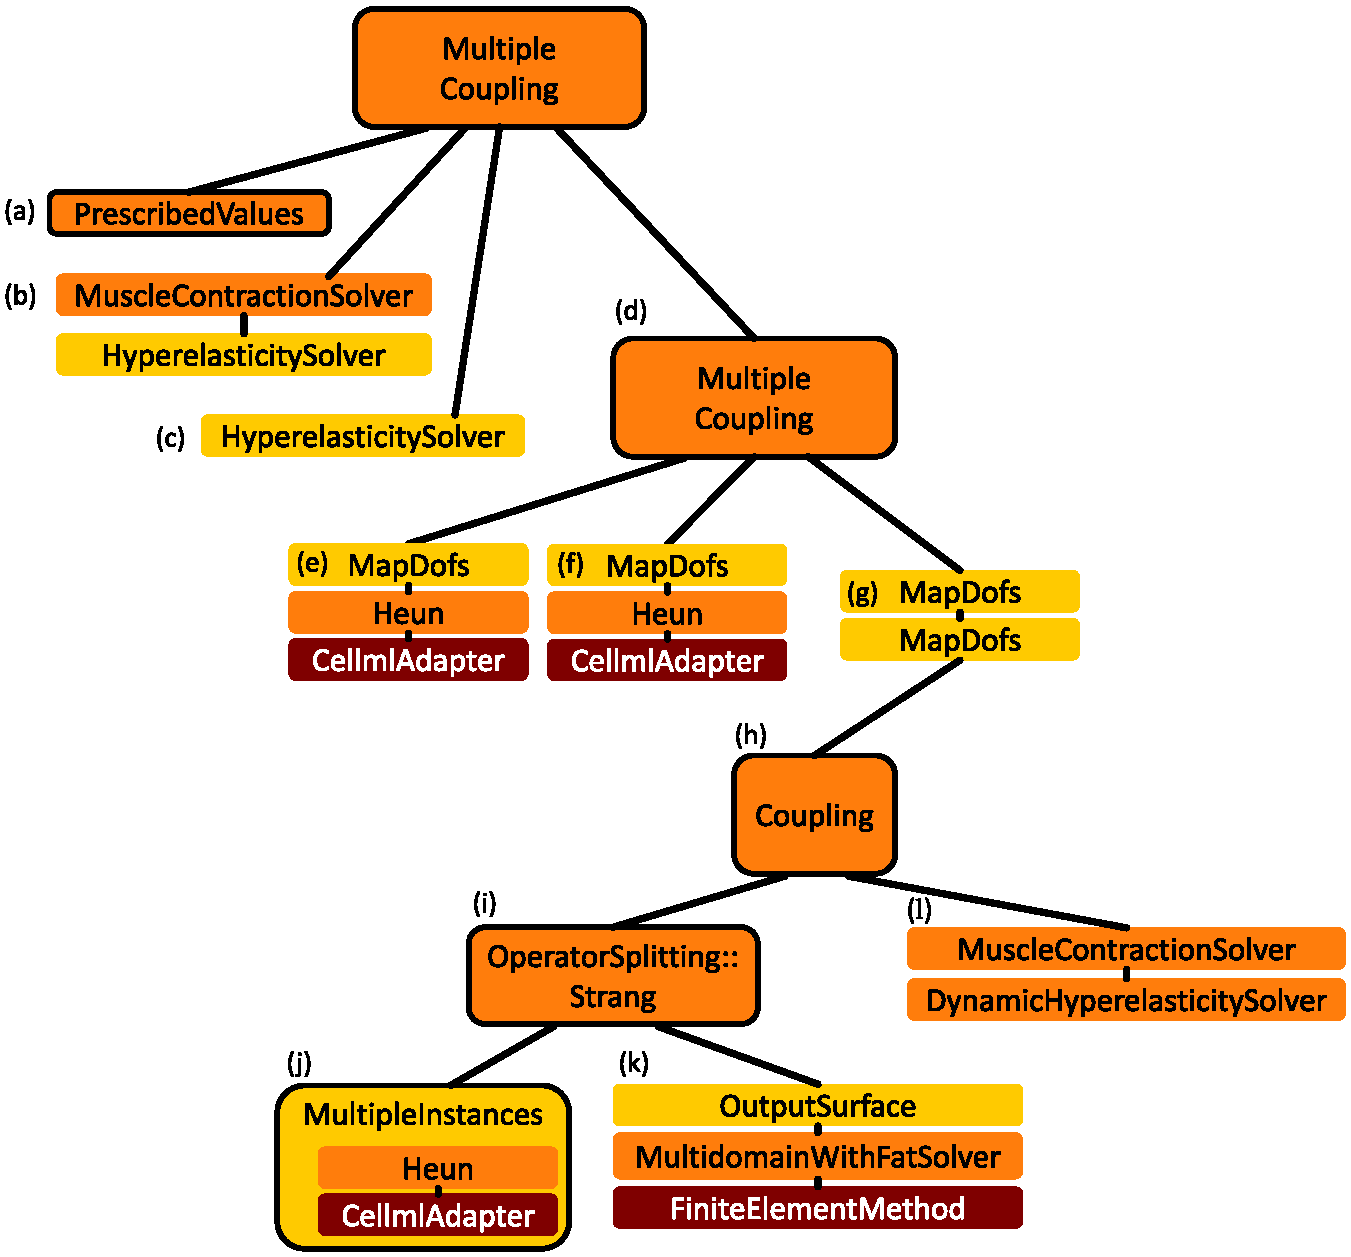
\includegraphics[width=0.9\textwidth]{images/implementation/solver_tree_multidomain_spindles.pdf}%
  \caption{Solver tree for a simulation of the neuromuscular system. Classes of type \code{DiscretizableInTime} are shown as red boxes, \code{TimeSteppingScheme}s are given by orange boxes.}%
  \label{fig:solver_tree_multidomain_spindles}%
\end{figure}

The following solver classes are involved in this example. For executing multiple solvers in series, the top-level \code{MultipleCoupling} class exists, which calls its nested solvers one by one in every timestep.
The \code{PrescribedValues} class (a) can be configured to set any of its field variables to prescribed values. The values can be set by callback functions in the python settings that get frequently called by the solver to update the values over time.

A \code{MuscleContractionSolver} combines either a static or a dynamic hyperelasticity model with the active stress term used in the muscle contraction model. The class in (b) uses the static \code{HyperelasticitySolver}. The solvers in (a) and (b) compute the static contraction of the muscle under a prescribed constant activation level. Then, another \code{HyperelasticitySolver} (c) stretches the muscle tissue again by a prescribed external force to yield a prestretched muscle. The actual transient simulation is then performed under the subtree at (d). 
Again, a \code{MultipleCoupling} class is used to run all nested solvers in every timestep.

In (e) and (f), two CellML models are solved using a Heun scheme, the first one for the muscle spindles and the second one for the motor neurons. A filter step is applied on the resulting signals and the values are copied to the destination field variables using the \code{MapDofs} class in (e), (f) and (g). A \code{MapDofs} class is able to copy degrees of freedom between two field variables, apply custom Python functions on the values and communicate values between processes in parallel execution.

The subtree under (h) is identical to the example presented in \cref{sec:exemplary_usage_2}. It solves the electrophysiology model using the multidomain equations in (j) and a subcellular model in (k), coupled to the solid mechanics model in (l).

The tree in \cref{fig:solver_tree_multidomain_spindles} consists of solver classes of different types. The orange boxes indicate timestepping schemes. Internally, these classes derive from a \code{TimeSteppingScheme} interface class. They have a common set of parameters such as the timestep width and end time.
The boxes with dark red background color are classes of type \code{DiscretizableInTime}. They represent a term or equation that can be nested in a timestepping scheme. There only exist two different classes of this type: The \code{CellmlAdapter}, which contains a system of DAEs given by a CellML model and the \code{FiniteElementMethod}, which discretizes the generalized Laplace operator $\div(\bfsigma \grad u)$.

Besides the classes of the presented example shown in \cref{fig:solver_tree_multidomain_spindles}, further solver classes are available in OpenDiHu. A comprehensive list of all available solver classes is given in the following section.

% summary of existing solvers additional solvers exist
\subsection{Summary of Existing Solver Classes}\label{sec:summary_of_existing_solver_classes}

All the timestepping schemes introduced in \cref{eq:ode_solver_schemes} are available to solve ODEs given by \code{Discretizable}\code{InTime} objects:
The explicit schemes are the explicit Euler and Heun's method. The available implicit schemes are the implicit Euler and Crank-Nicolson method.
Implemented operator splitting schemes are the Godunov and Strang splittings. The implementation of the \code{Coupling} class is identical to Godunov splitting.
As mentioned in \cref{sec:exemplary_usage_3}, \code{DiscretizableInTime} objects are either given by the \code{CellmlAdapter} or the \code{FiniteElementMethod.}

Some classes are special solvers for dedicated models: A \code{StaticBidomainSolver} is used to solve the first bidomain equation \cref{eq:bidomain1}. The \code{Multidomain}\code{Solver} and \code{Multidomain}\code{WithFatSolver} classes solve the multidomain models \cref{eq:multidomain1,eq:multidomain2} without and with body fat domain. A class \code{FastMonodomainSolver} exists that improves the parallel performance of the fiber based electrophysiology solver using the monodomain equation \cref{eq:monodomain}.

Solid mechanics models can be computed by a series of specialized solvers. The \code{QuasiStaticLinearElasticitySolver} class uses a \code{FiniteElementMethod} object to compute 3D linear elasticity using Hooke's Law with an additional active stress term, as derived in \cref{sec:linearized_mechanics_model}. The \code{HyperelasticitySolver} class solves the static hyperelasticity formulation for any material model, as presented in \cref{sec:static_hyperelastic_fe_model}. The \code{DynamicHyperelasticitySolver} class inherits from the \code{HyperelasticitySolver} class and adds functionality to solve the dynamic hyperelasticity formulation shown in \cref{sec:solver_dynamic_hyperelasticity_fe_model}. 
Both the static and the dynamic hyperelastic solvers do not incorporate the active stress term that is present in the muscle contraction model. This is handled by another class, the \code{MuscleContractionSolver}. It uses either a \code{HyperelasticitySolver} or a \code{DynamicHyperelasticitySolver} object and adds the functionality accordingly.

Instead of solving a model numerically, also precalculated analytic solutions can be used. This can be done using the \code{PrescribedValues} class, which uses a Python function to set the solution values. Further auxiliary classes exist that are no numeric solver: The \code{MapDofs} class gives flexibility to transfer certain degrees of freedom between field variables. The \code{Dummy} class can be used as a placeholder. The \code{OutputSurface} class extracts a 2D mesh at the surface of a 3D mesh and writes it to an output file using the normal output writers. This can be used to reduce the amount of data output for finely resolved EMG simulations, where only the values at the surface are of interest.

Moreover, adapters to external software tools are implemented. The class \code{Nonlinear}\code{ElasticitySolverFebio} allows to use the solver \emph{FEBio} \cite{Maas2012,maas2017febio} for solving a continuum mechanics model and couple it to an electrophysiology model in OpenDiHu.
Two adapters to the numerical coupling library preCICE \cite{precice}, \code{PreciceAdapter} and \code{PreciceAdapterVolumeCoupling} exist for surface and volume coupling. They can be configured to implicitely or explicitely couple any field variables to external solvers or to couple two separate instances of OpenDiHu.
% summary structure, how to define the settings, help with gui program
For more details on the solver classes and their configuration, we refer to the online documentation \cite{opendihuWeb}.

\subsection{Graphical Helper Program}
For the creation of new examples from scratch, a helper program with a graphical user interface exists. The program was created by Matthias Tompert in his Bachelor thesis and is included in the OpenDiHu repository under \code{scripts/gui/gui.py}.

Graphical widgets allow to select and nest compatible solver classes for OpenDiHu. The corresponding Python settings are automatically shown with their default values and can be adjusted in the graphical user interface. For every option, explanatory comments are displayed and buttons allows to open the corresponding page of the online documentation in a web browser.

The program also features a horizontally split code editor, which shows both the C++ code and the corresponding Python code for the settings, either for a single node in the solver tree or as a global view of the whole example. 
After the user completes the adjustments of the solver structure and the settings, the C++ source file and the Python settings can be exported and used with OpenDiHu.

The program is also capable of parsing existing C++ and Python files and, thus, loading an existing example into the graphical representation to be extended by the user. The program is able to parse a large portion of the solvers and options that are available in OpenDiHu. However, some more advanced examples, e.g., where the Python settings contain complex code constructs are not fully supported.

\Cref{fig:gui_a} shows the user interface after the 2D diffusion example of OpenDiHu has been loaded. The left pane in \cref{fig:gui} represents the solver tree as it appears in the C++ file. The right pane in \cref{fig:gui} displays the settings for the selected item in the left pane, which, in this case, is the mesh. Additional options that are not yet present in the Python settings are grayed out and can be added by clicking the checkboxes.
\Cref{fig:gui3} shows an alternative view in the right pane, which displays the corresponding Python code. The user can also directly edit the settings there.

\begin{figure}%
  \centering%
  \begin{subfigure}[t]{0.71\textwidth}%
    \centering%
    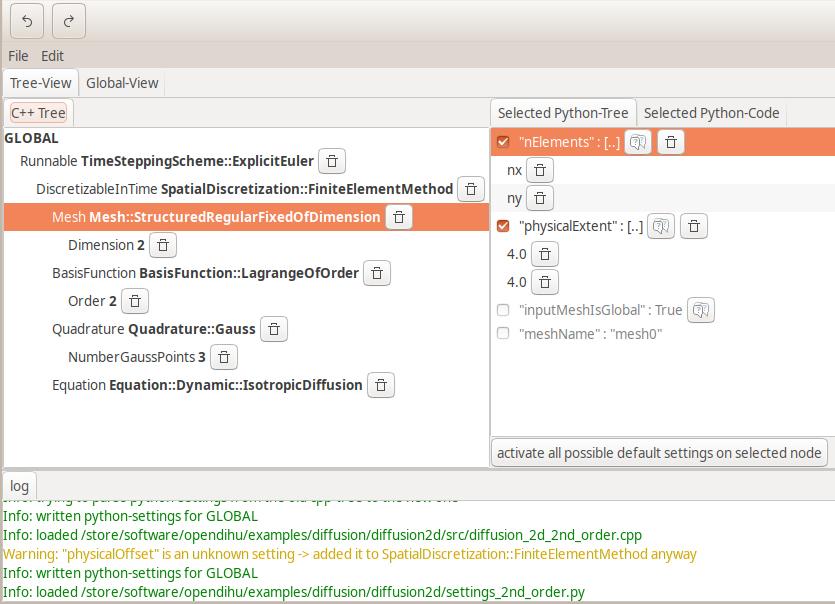
\includegraphics[height=8cm]{images/implementation/gui.png}
    \caption{User interface with the tree of nested solvers on the left and the Python settings for the selected mesh on the right.}%
    \label{fig:gui}%
  \end{subfigure}
  \,
  \begin{subfigure}[t]{0.27\textwidth}%
    \centering%
    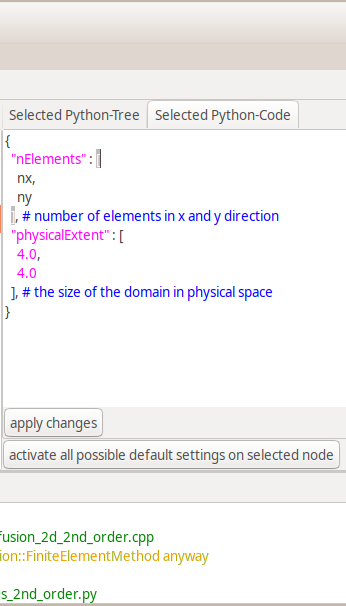
\includegraphics[height=8cm]{images/implementation/gui3.png}
    \caption{Alternative view of the right pane that shows the Python settings editor.}%
    \label{fig:gui3}%
  \end{subfigure}
  \caption{Graphical helper program to create and adjust the C++ and Python codes of OpenDiHu examples.}%
  \label{fig:gui_a}%
\end{figure}%



